\documentclass[12pt,a4paper]{article}
\topmargin -1.6cm
\addtolength{\textheight}{4cm}
\textwidth  15.5cm

\leftmargin      5mm
\rightmargin     5mm
\oddsidemargin   5mm
\evensidemargin  5mm

\usepackage{hyperref}
\usepackage{polski}
\usepackage[utf8]{inputenc}
\usepackage{graphicx}
\usepackage{units}
\usepackage{sty/style}
\usepackage{float}

\projekt{Modelowanie i identyfikacja}
\autor{Marcin Bober, 249426}
\przedmiot{Identyfikacja i modelowanie statystyczne}
\prowadzacy{Mgr inż. Maciej Filiński}

\begin{document}
\pdfpageheight   297mm
\pdfpagewidth    210mm

\StronaTytulowa
\SpisTresci

\pagebreak

\section{Generator liczb pseudolosowych}
  \subsection{Opis}
  Zadanie polega na implementacji generatora liczb pseudolosowych z rozkładu jednostajnego oraz analizie wyników uzyskanych z jego udziałem. Generator oparty jest na przekształceniu piłokształtnym o równaniu $X_{n+1} = X_n \cdot z - [X_n \cdot z]$ 

  \subsection{Wpływ wartości początkowej X na własności generatora}

  Wartość $Z$ ustawiona została na wartość 51. Wykorzystano 1000 próbek.

  \begin{figure}[H]
    \centering
    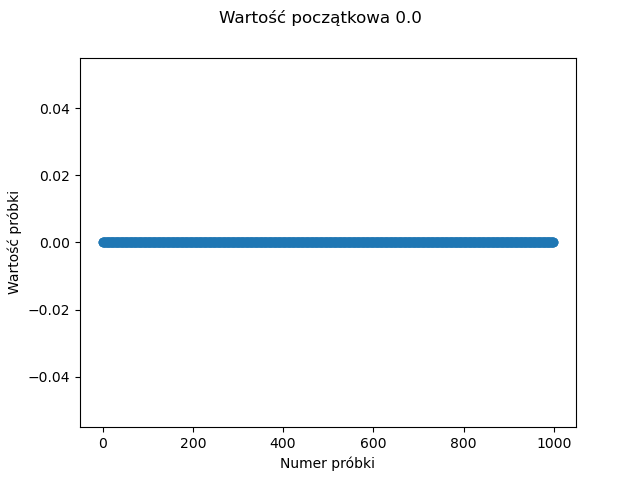
\includegraphics[height=0.3\textheight]{figures/Figure_1.png}
    \label{fig:1}
  \end{figure}

  \begin{figure}[H]
    \centering
    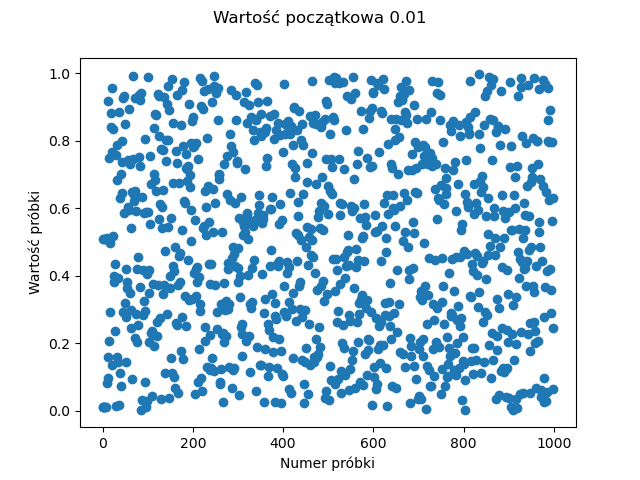
\includegraphics[height=0.3\textheight]{figures/Figure_2.png}
    \label{fig:2}
  \end{figure}

  \begin{figure}[H]
    \centering
    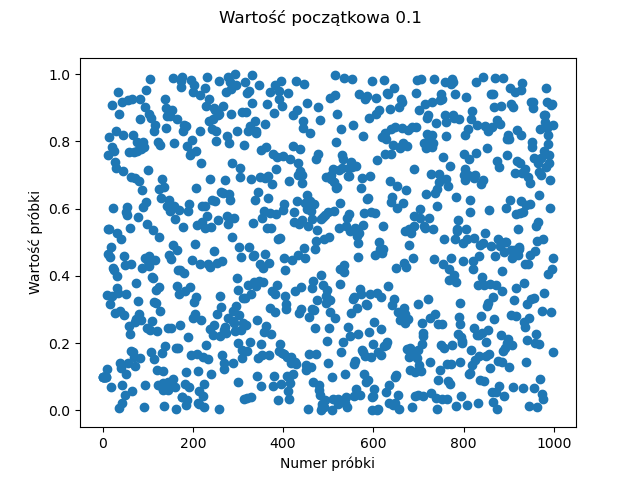
\includegraphics[height=0.3\textheight]{figures/Figure_3.png}
    \label{fig:3}
  \end{figure}

  \begin{figure}[H]
    \centering
    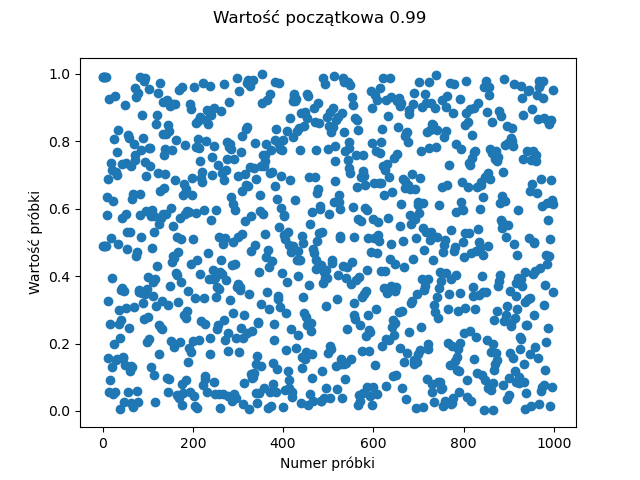
\includegraphics[height=0.3\textheight]{figures/Figure_4.png}
    \label{fig:4}
  \end{figure}

  \begin{figure}[H]
    \centering
    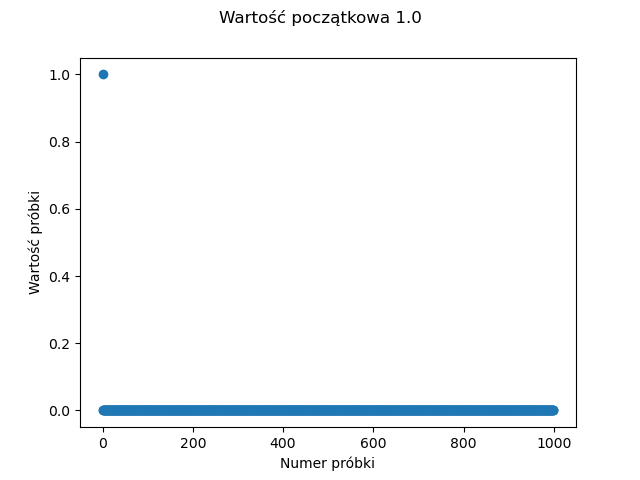
\includegraphics[height=0.3\textheight]{figures/Figure_5.png}
    \label{fig:5}
  \end{figure}
  
  \begin{itemize}
    \item Ustawienie wartości początkowej równej zero powoduje że wszystkie wygenerowane próbki są zerowe. (Patrz wykres \ref{fig:1}) Dzieje się tak ponieważ algorytm opiera się o obliczenie iloczynu liczb, których jednym ze składników jest zero.
    \item Wybór liczby całkowitej spowoduje że pierwsza próbka jest równa tej wartości, a wszystkie kolejne są zerowe (Patrz wykres \ref{fig:5}). Wynika to z faktu że obliczana jest reszta z dzielenia wartości przez jeden, która w taki wypadku zawsze równa jest zero.
    \item Zalecanym zakresem wyboru wartości początkowej jest przedział zawierający liczby większe od zera, z pominięciem liczb całkowitych.
  \end{itemize}

  \subsection{Wpływ parametru Z na własności generatora}

  Wartość $X_0$ ustawiona została na wartość 0,01. Wykorzystano 1000 próbek.

  \begin{figure}[H]
    \centering
    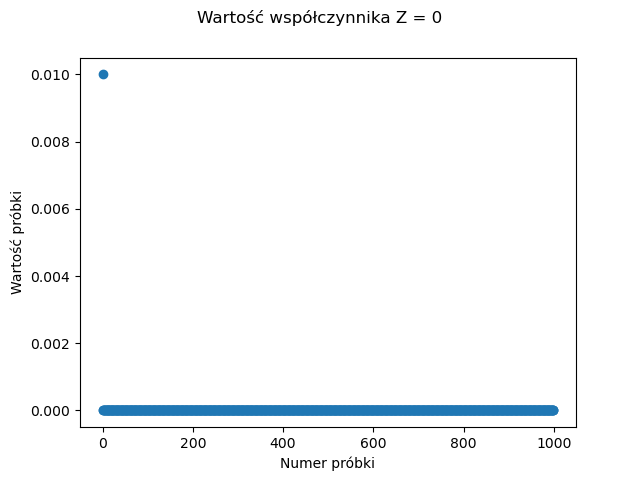
\includegraphics[height=0.3\textheight]{figures/Figure_6.png}
    \label{fig:6}
  \end{figure}

  \begin{figure}[H]
    \centering
    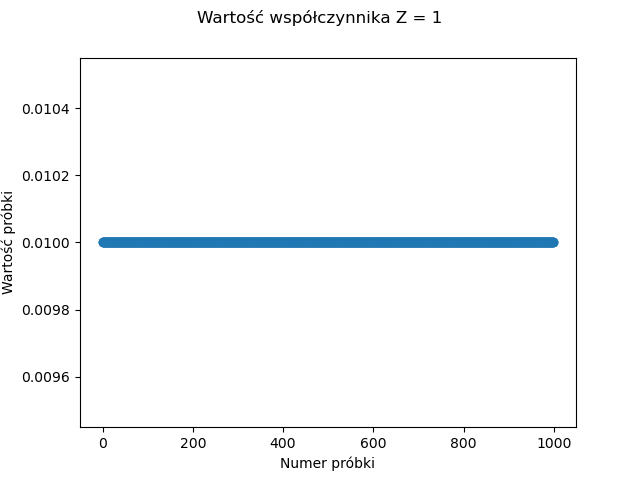
\includegraphics[height=0.3\textheight]{figures/Figure_7.png}
    \label{fig:7}
  \end{figure}

  \begin{figure}[H]
    \centering
    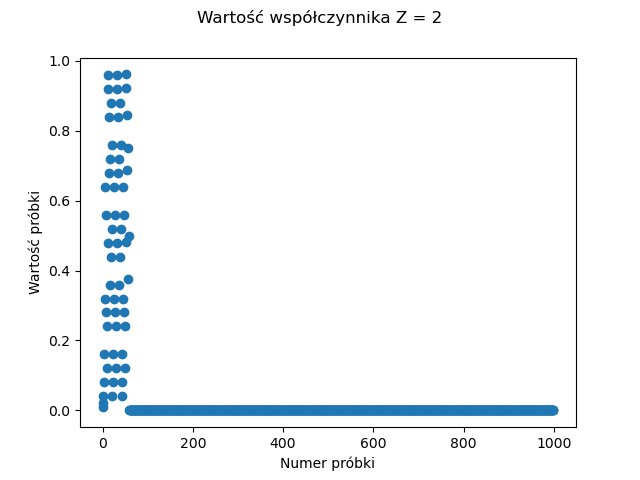
\includegraphics[height=0.3\textheight]{figures/Figure_8.png}
    \label{fig:8}
  \end{figure}

  \begin{figure}[H]
    \centering
    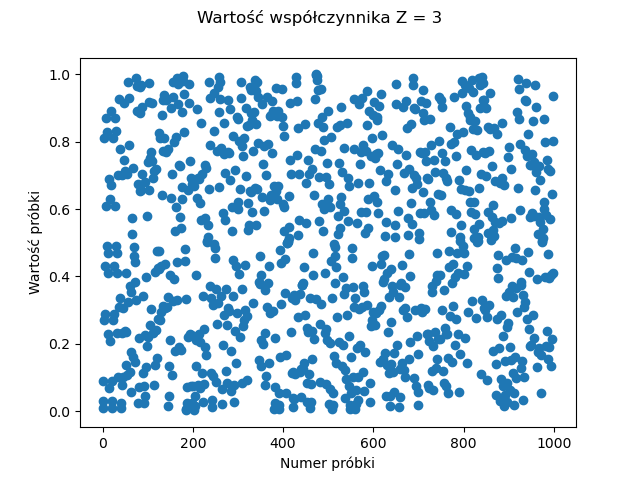
\includegraphics[height=0.3\textheight]{figures/Figure_9.png}
    \label{fig:9}
  \end{figure}
  
  \begin{itemize}
    \item Dla zerowego współczynnika $Z$ pierwsza próbka uzyskuje wartość początkowa, a kolejne są zerami. Wynika to z mnożenia tych wyników przez współczynnik $Z$ czyli zero.
    \item Gdy wartość $Z$ jest równa jedności, wszystkie otrzymane wyniki są identyczne z wartością startową.
    \item W przypadku wykorzystania liczb parzystych, uzyskiwane wyniki szybko trafiają na wartość zero, która powoduje zatrzymanie generowania kolejnych wartości losowych. 
    \item Najlepsze wyniki otrzymywane są dla współczynnika $Z$ będącego dużą liczbą pierwszą. 
  \end{itemize}

  \subsection{Okres generatora dla wybranych wartości Z}

  \begin{table}[h!]
    \centering
    \begin{tabular}{ c | c | c }
      $X_0$ & $Z$ & okres generatora  \\ 
      \hline
      0,1 & 1 & 1  \\  
      0,1 & 2 & 4  \\  
      0,1 & 3 & 4  \\  
      0,1 & 4 & 2  \\  
      0,1 & 5 & 1  \\
      0,1 & 6 & 1  \\
      0,1 & 7 & 4  \\
      0,1 & 8 & 4 
    \end{tabular}
    \caption{Nastawy PD i odpowiadający im rząd błędu.}
    \label{table:1}
  \end{table}

  \subsection{Podobieństwo histogramu ciągu wygenerowaych liczb, a gęstość rozkładu jednostajnego}


  \begin{figure}[H]
    \centering
    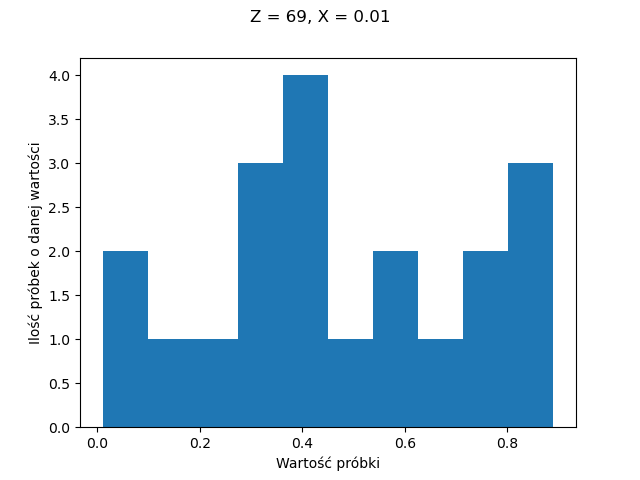
\includegraphics[height=0.25\textheight]{figures/Figure_10.png}
    \caption{Ilość wygenerowanych próbek - 20}
    \label{fig:10}
  \end{figure}

  \begin{figure}[H]
    \centering
    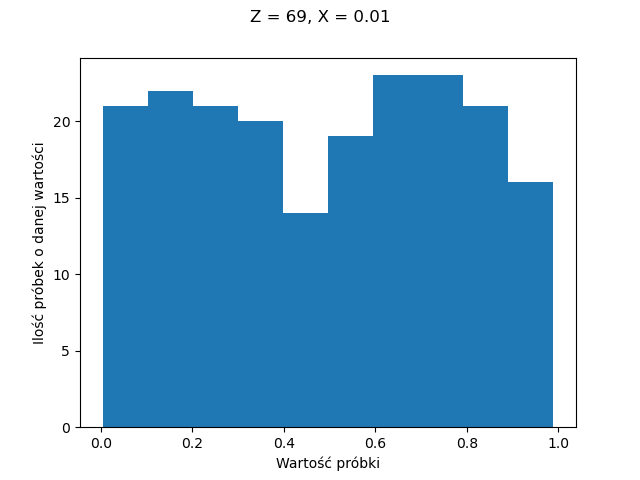
\includegraphics[height=0.25\textheight]{figures/Figure_11.png}
    \caption{Ilość wygenerowanych próbek - 200}
    \label{fig:11}
  \end{figure}

  \begin{figure}[H]
    \centering
    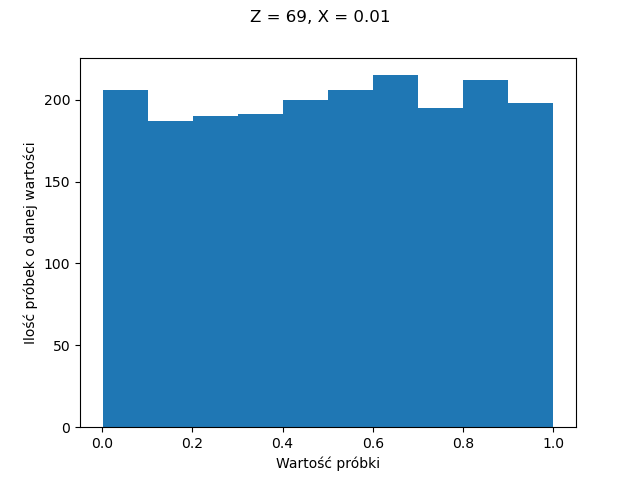
\includegraphics[height=0.25\textheight]{figures/Figure_12.png}
    \caption{Ilość wygenerowanych próbek - 2000}
    \label{fig:12}
  \end{figure}

  \begin{figure}[H]
    \centering
    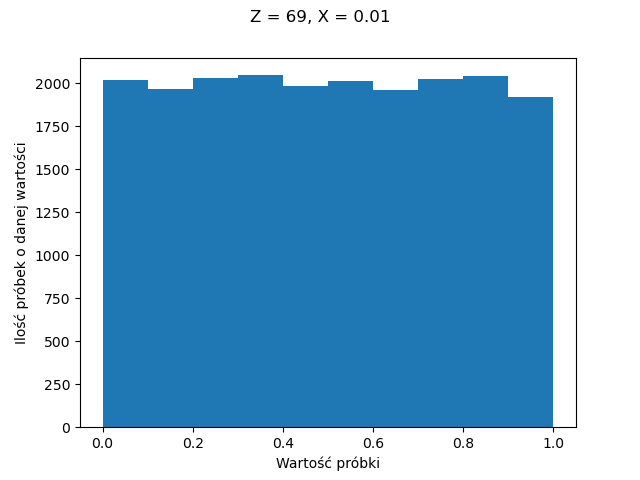
\includegraphics[height=0.25\textheight]{figures/Figure_13.png}
    \caption{Ilość wygenerowanych próbek - 20000}
    \label{fig:13}
  \end{figure}


\section{Podsumowanie}

\end{document}